
%% ============================================================
%% PŘÍKLAD 2E
%% ============================================================
\section{Příklad 2E -- Osový kvadratický moment nesymetrického průřezu}

\subsection{Zadání}

U~tělesa podle obrázku určete osový kvadratický moment k~ose $x$ a~$y$. Střední hodnoty rozměrů jsou uvedeny na obrázku, variační koeficient $\mathrm{\nu} = 0{,}2$. Stochastické veličiny popisujte normálním rozdělením.

\subsection{Geometrie průřezu}

Jedná se o nesymetrický průřez složený ze tří obdélníků odpovídajících horní pásnici, stojině a dolní pásnici (Obrázek 1, rozlišeno šrafami). Počátek souřadného systému se nachází v~levém dolním rohu tělesa. Rozměry průřezu jsou zobrazeny v tabulce 1. Šířka stojiny byla uvažována jako X1.

\begin{figure}[htbp]
    \centering
    
    % ---- First minipage for the Picture ----
    \begin{minipage}[c]{0.6\textwidth}
        \centering
        % Replace 'example-image' with your actual image file name
        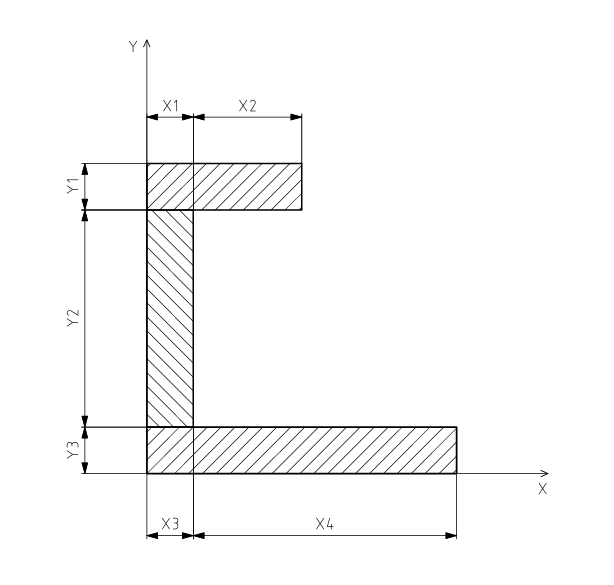
\includegraphics[width=\textwidth]{size.png}
        \caption{Průřez tělesa}
        \label{fig:my_picture}
    \end{minipage}
    \hfill % Adds flexible space between the two minipages
    % ---- Second minipage for the Table ----
    \begin{minipage}[c]{0.3\textwidth}
        \centering
        \captionof{table}{Rozměry průřezu}
        \label{tab:my_table}
        \begin{tabular}{lccccc}
\toprule
\textbf{Rozměr} & $\boldsymbol{l}$ [mm] & $\boldsymbol{\nu}$ [-]  \\
\midrule
X1  & 30 & 0,2  \\
X2  & 70 & 0,2  \\
X3  & 30 & 0,2  \\
X4  & 170 & 0,2 \\
Y1  & 30 & 0,2  \\
Y2  & 140 & 0,2  \\
Y3  & 30 & 0,2  \\
\bottomrule
\end{tabular}
    \end{minipage}
    
\end{figure}

 \newpage

\subsection{Řešení}

\subsubsection{Osové kvadratické momenty}
Pro osový kvadratický moment obdélníku platí: 
\begin{equation}
    I =  \frac{b_i}{3}  \cdot (h_i^3-L^3)  
\end{equation}
kde b odpovídá délce strany rovnoběžné s osou, h odpovídá délce strany kolmé na osu a L odpovídá vzdálenosti obdélníku od osy. 

Osový kvadratický moment tělesa, složeného z více obdélníků, pak odpovídá součtu jejich osových kvadratických momentů.

Na základě vzorce 1 lze vyjádřit kvadratický moment pro jednotlivé obdélníky k ose X jako:
\\ 
 \\ 
Horní pásnice:
\begin{equation}
    I_{x3} =  \frac{1}{3}  \cdot(X1 + X2) \cdot ((Y1 + Y2 + Y3)^3 - (Y2 + Y3)^3)
\end{equation}
Stojina:
\begin{equation}
    I_{x2} =  \frac{1}{3}  \cdot X1 \cdot ((Y3 + Y2)^3 - Y3^3) 
\end{equation}
Dolní pásnice:
\begin{equation}
    I_{x1} =  \frac{1}{3}  \cdot (X3 + X4) \cdot Y3^3 
\end{equation}
Celkový osový kvadratický moment:
\begin{equation}
    I_x =  \sum_{i=1}^{3}  I_{xi}
\end{equation}
 
a k ose Y jako:
\\ 
 \\ 
\noindent Horní pásnice:
\begin{equation}
    I_{y1} =  \frac{1}{3}  \cdot Y1 \cdot  (X1 + X2)^3  
\end{equation}
Stojina:
\begin{equation}
    I_{y2} =  \frac{1}{3}  \cdot Y2 \cdot X1^3
\end{equation}
Dolní pásnice:
\begin{equation}
    I_{y3} =  \frac{1}{3}  \cdot Y3 \cdot (X3 + X4)^3
\end{equation}
Celkový osový kvadratický moment:
\begin{equation}
    I_y =  \sum_{i=1}^{3} I_{yi}
\end{equation}

\subsubsection{ Zpracování metodou Monte Carlo}

Rozměrové veličiny  jsou popsány normálním rozdělením s~$\mathrm{\nu} = 0{,}2$. Pro potřeby numerického řešení metodou Monte Carlo byly v programu Matlab R2024B vygenerovány statistické soubory o počtu prvků $N = 1\E{8}$ pro každou z nich. 
Na jejich základě byly vypočítány střední hodnoty kvadratických osových momentů k oběma osám, jejich směrodatné odchylky a variační koeficienty. Ty zobrazuje tabulka 2.


\begin{table}[H]
\centering
\caption{Statistické charakteristiky osových kvadratických momentů }
\begin{tabular}{lcccc}
\toprule
\textbf{Veličina} & $\boldsymbol{\mu}$ [$\E{6}$ mm$^4$] & $\boldsymbol{\sigma}$ [$\E{6}$ mm$^4$] & $\boldsymbol{\nu}$ [-] \\
\midrule
$I_{x}$ & 161{,}10 & 68{,}21 & 0{,}423  \\
$I_{y}$ & 99{,}26 & 48{,}34 & 0{,}487  \\
\bottomrule
\end{tabular}
\end{table}

\noindent Variační koeficienty výstupu ($0{,}42$--$0{,}49$) jsou oproti vstupu ($0{,}2$) více než dvojnásobné, to je dáno jejich závislostí na rozměrech ve třetí mocnině (zesílení nejistoty). 

Histogramy pro oba statistické soubory osových kvadratických momentů zobrazuje obrázek 2. Důvodem pro jejich asymetrii je opět třetí mocnina vstupů.


\begin{figure}[htbp]
    \centering
    
    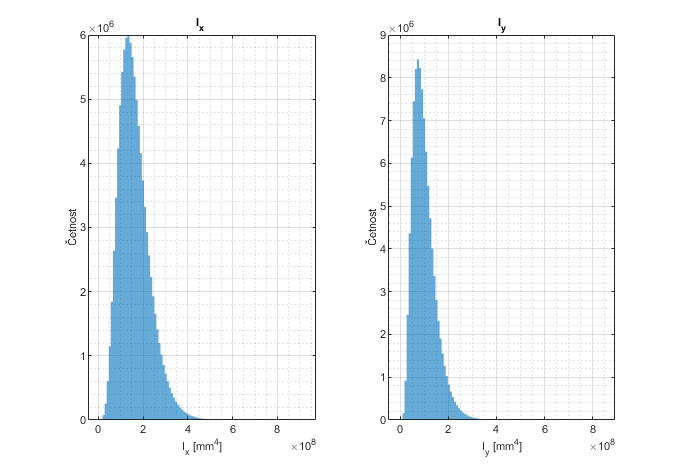
\includegraphics[width=0.8\textwidth]{histo.png} 
    \caption{Histogramy osových kvadratických momentů z Monte Carlo}
    \label{fig:single_picture}
\end{figure}
Srovnání obou statistických souborů normalizovaných s pomocí hustoty pravděpodnosti je vykresleno na obrázku 3.
\begin{figure}[htbp]
    \centering
    
    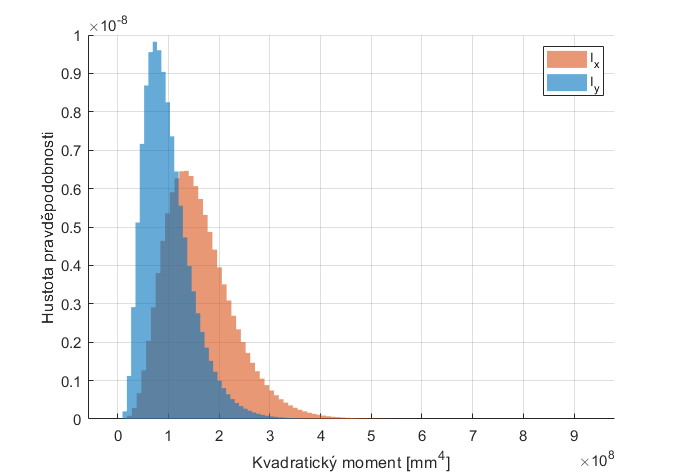
\includegraphics[width=0.7\textwidth]{hustoty.png} 
    \caption{Srovnání hustot pravděpodobnosti osových kvadratických momentů}
    \label{fig:single_picture}
\end{figure}
